\chapter{Alternative compositions}
\label{sec:comps}

Up until this point we have looked in detail at the high-entropy silicide \ch{(CrFeMnNi)Si2}. In this chapter we will broaden our search of compositions based on the $\beta$-\ch{FeSi2} structure. First, we will look at various compositions inside the quaternary phase diagram of Cr, Fe, Mn and Ni, then consider some compositions where chromium, manganese or nickel are replaced by cobalt or titanium. 

\section{Exploring the quaternary phase diagram}
In this section, we aim to expand our search of this diagram by generating SQSs of the 48 atom model slightly away from equimolar distribution of 3d elements. The list of compositions are listed in table 8.1, with corresponding total energy, magnetic moment and formation energy in the familiar format. Ideally each composition would differ only by one element to provide a clear view of each direction in the phase diagram, but the TDEP implementation insisted in also reducing Nickel to stay consistent with the 48 atom supercell. 

\begin{table}[H]
\centering
\begin{tabular}{@{}cccccc@{}}
\toprule
Composition           & \multicolumn{2}{c}{\begin{tabular}[c]{@{}c@{}}Toten\\ (eV)\end{tabular}} & \multicolumn{2}{c}{\begin{tabular}[c]{@{}c@{}}Mag \\ ($\mu_B$) \end{tabular}} & \begin{tabular}[c]{@{}c@{}}$E_{FPA}$\\ (eV) \end{tabular} \\ \midrule
                      & mean                                 & std                               & mean                                 & std                                 & mean                                                      \\ \midrule
\ch{Cr3Fe3Mn7Ni3Si32} & - 6.695                             & 0.004                            & 0.138                               & 0.019                              & -0.300                                                  \\
\ch{Cr5Fe5Mn3Ni3Si32} & - 6.671                             & 0.003                            & 0.113                               & 0.022                              & -0.286                                                  \\
\ch{Cr5Fe3Mn5Ni3Si32} & - 6.685                             & 0.004                            & 0.138                               & 0.046                              & -0.271                                                  \\
\ch{Cr3Fe5Mn5Ni3Si32} & - 6.680                             & 0.004                            & 0.094                               & 0.021                              & -0.315                                                  \\
\ch{Cr3Fe3Mn3Ni7Si32} & - 6.392                             & 0.008                            & 0.016                               & 0.010                              & -0.285                                                  \\ \bottomrule
\end{tabular}
\caption{Total energy, magnetic moment and formation energy of various compositions of the Cr:Fe:Mn:Ni:Si system.}
\end{table}


In table 8.1 we observe that moving away from the equimolar system result in both less and more stable alloys. Clearly the lowest formation energies (most stable) correspond to compositions rich in manganese and poor in chromium. Likewise the least stable compositions in table 8.1 contain either increased amounts of Cr or reduced amounts of Mn compared to the equimolar system. In the equimolar composition the magnetic moment was attributed to primarily Cr and Mn atoms in the lattice. In table 8.1 we observe similarly that compositions rich in Cr and Mn exhibits the largest magnetic moments and vice versa. The band gaps of the respective compositions in five unique SQSs can be seen in table 8.2 below, calculated with PBE GGA.   

\begin{table}[H]
\centering
\begin{tabular}{@{}ccccc@{}}
\toprule
Composition                                                 & SQS        & \begin{tabular}[c]{@{}c@{}}$E_G ^\text{up, eigen}(0.5)$\\ (eV)\end{tabular} & \begin{tabular}[c]{@{}c@{}}$E_G ^\text{dw, eigen}(0.5)$\\ (eV)\end{tabular} & \begin{tabular}[c]{@{}c@{}}$E_G ^\text{tot, eigen}(0.5)$\\ (eV)\end{tabular} \\ \midrule
\multicolumn{1}{c|}{\multirow{5}{*}{\ch{Cr3Fe3Mn7Ni3Si32}}} & A          & 0.339                                                                      & 0                                                                           & 0                                                                                 \\
\multicolumn{1}{c|}{}                                       & \textbf{B} & 0.475                                                                      & 0                                                                           & 0                                                                                 \\
\multicolumn{1}{c|}{}                                       & C          & 0.134                                                                      & 0                                                                           & 0                                                                                 \\
\multicolumn{1}{c|}{}                                       & D          & 0.195                                                                      & 0.006                                                                      & 0.006                                                                            \\
\multicolumn{1}{c|}{}                                       & E          & 0.421                                                                      & 0                                                                           & 0                                                                                 \\ \midrule
\multicolumn{1}{c|}{\multirow{4}{*}{\ch{Cr5Fe5Mn3Ni3Si32}}} & A          & \textit{0.003}                                                              & 0                                                                           & 0                                                                                 \\
\multicolumn{1}{c|}{}                                       & \textbf{C} & \textit{0.210}                                                               & 0                                                                           & 0                                                                                 \\
\multicolumn{1}{c|}{}                                       & D          & 0.067                                                                      & 0.041                                                                      & 0.037                                                                            \\
\multicolumn{1}{c|}{}                                       & E          & \textit{0.362}                                                              & 0                                                                           & 0                                                                                 \\ \midrule
\multicolumn{1}{c|}{\multirow{5}{*}{\ch{Cr5Fe3Mn5Ni3Si32}}} & \textbf{A} & 0.208                                                                      & 0                                                                           & 0                                                                                 \\
\multicolumn{1}{c|}{}                                       & B          & 0.405                                                                      & 0                                                                           & 0                                                                                 \\
\multicolumn{1}{c|}{}                                       & C          & 0.466                                                                      & 0                                                                           & 0                                                                                 \\
\multicolumn{1}{c|}{}                                       & D          & 0.084                                                                      & 0.012                                                                      & 0.012                                                                            \\
\multicolumn{1}{c|}{}                                       & E          & 0.301                                                                      & 0                                                                           & 0                                                                                 \\ \midrule
\multicolumn{1}{c|}{\multirow{4}{*}{\ch{Cr3Fe5Mn5Ni3Si32}}} & A          & 0.392                                                                      & 0                                                                           & 0                                                                                 \\
\multicolumn{1}{c|}{}                                       & C          & 0.129                                                                      & 0                                                                           & 0                                                                                 \\
\multicolumn{1}{c|}{}                                       & \textbf{D} & 0.260                                                                      & 0.100                                                                      & 0.100                                                                            \\
\multicolumn{1}{c|}{}                                       & E          & 0.359                                                                      & 0.100                                                                      & 0.085                                                                            \\ \midrule
\multicolumn{1}{c|}{\multirow{5}{*}{\ch{Cr3Fe3Mn3Ni7Si32}}}    & A          & 0                                                                           & 0                                                                           & 0                                                                                 \\
\multicolumn{1}{c|}{}                                       & B          & 0                                                                           & 0                                                                           & 0                                                                                 \\
\multicolumn{1}{c|}{}                                       & C          & 0                                                                           & 0                                                                           & 0                                                                                 \\
\multicolumn{1}{c|}{}                                       & D          & 0                                                                           & 0                                                                           & 0                                                                                 \\
\multicolumn{1}{c|}{}                                       & \textbf{E} & \textit{0.040}                                                               & 0                                                                           & 0                                                                                 \\ \bottomrule 
\end{tabular}
\caption{Band gaps of various compositions of \ch{(CrFeMnNi)Si2}. Most stable SQS of a set is highlighted in bold text, defect/impurity band gaps are listed in $italic$. Some SQSs were excluded from the table due to unsuccessful calculations.}
\end{table}

From table 8.2 we observe that most compositions are half-metals like the equimolar system with a spin up polarization. Each composition shows large variation between configurations. We note $E_\text{G, max} ^\text{up} \approx 0.5$ eV and $E_\text{min} ^\text{up} \approx 0.1$ eV in both \ch{Cr3Fe3Mn7Ni3Si32} and \ch{Cr5Fe3Mn5Ni3Si32}, and further $E_\text{G, max} ^\text{up} \approx 0.4$ eV and $E_\text{min} ^\text{up} \approx 0.1$ eV in \ch{Cr3FeMn5Ni3Si32}. In all three of these compositions the proportion of manganese is increased relative to the equimolar system, and two out of the three compositions contain reduced amounts of chromium. Looking at the two compositions with the least indication of a band gap \ch{Cr5Fe5Mn3Ni3Si32} and \ch{Cr3Fe3Mn3Ni7}, these contain reduced amounts of manganese. Thus, based on the few compositions tested in this experiment we can state a relation of the band gap mainly to manganese, but also chromium.     

Based on the most stable configuration of each composition, we observe very encouraging results in the \ch{Cr3Fe3Mn7Ni3Si32} composition with the largest $E_G ^\text{up}$ of the set of configurations. Likewise the most stable SQS of the \ch{Cr3Fe5Mn5Ni3Si32} composition is a semiconductor with a total band gap of about 0.1 eV. In the composition \ch{Cr5Fe5Mn3Ni3Si32}, the most stable SQS predicts a defect or impurity band gap as we discussed previously where the eigenvalues return a finite band gap despite of defect states. However we have not been able to investigate the nature and effect of this impurity band gap to further extent, likewise for the similar impurity gaps listed in table 8.2 and the 0 band gaps in spin down. Below in figures 8.1 and 8.2 we include the projected density of states around $E_F$ of the most stable SQS of each composition. Because we only include and discuss the most stable SQS, the features of these figures can be subject to the uniqueness of that particular SQS rather than a distinct feature of the exact composition, however as stated previously the most stable configuration provides the most likely properties of the composition within the scope of this project. 

\begin{figure}[H]
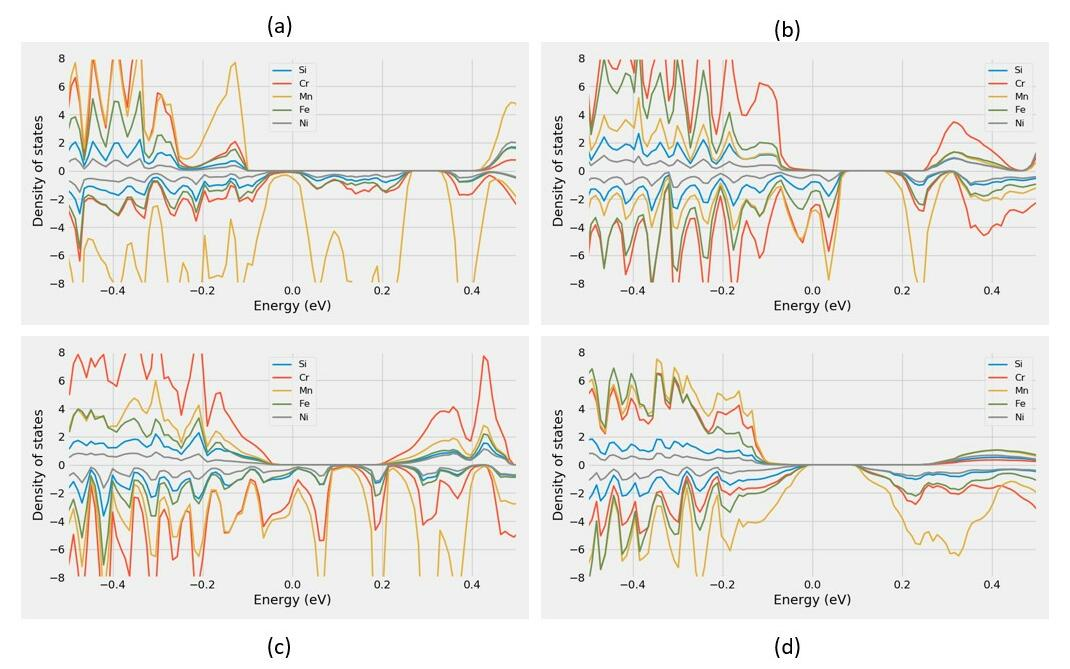
\includegraphics[width=\linewidth]{results/fesi2/permutations/perm_LDOS_crop.jpg}
\caption{Projected density of states [states/eV] of (a) \ch{Cr3Fe3Mn7Ni3Si32} (SQS B), (b) \ch{Cr5Fe5Mn3Ni3Si32} (SQS C), (c) \ch{Cr5Fe3Mn5Ni3Si32} (SQS A), (d) \ch{Cr3Fe5Mn5Ni3Si32} (SQS D)}
\end{figure}

The PDOSs is in good agreement with the listed values in table 7.2. \ch{Cr3Fe3Mn7Ni3Si32}  and \ch{Cr5Fe3Mn5Ni3Si32} both display sizable band gaps in spin, while figure 8.1 d point to a total band gap around 0.1 eV for SQS D of \ch{Cr3Fe5Mn5Ni3Si32}. On the other hand we observe as for the 192-atom SQS a dissimilarity between the density of states band gap in \ch{Cr5Fe5Mn3Ni3Si32} SQS C (figure 8.1 b) and the eigenvalue (impurity) band gap listed in table 7.2. This can be better understood by figure A.3 in appendix A.1 that clearly show small finite values at $E_F$ in spin up. This DOS may resemble that of a doped material.    


In figure 7.7 we observed that manganese distinctly occupied states in the spin down channel around $E_F$ and was a key contributor as to why the spin down channel of \ch{(CrFeMnNi)Si2} was metallic in the most stable SQS. This is also largely the case in the compositions shown above in figure 8.1 and 8.2, and is particularly evident in figure 8.1 where Mn dominates the spin down states around $E_F$ in the \ch{Cr3Fe3Mn7Ni3Si32} composition. By reducing the number of Mn we still find that the Mn states prohibit the band gap in spin down, as seen in figure 8.1 b. In the chromium rich compositions plotted in figures 8.1 b and c, we observe that also Cr states prohibit the spin down band gap, and dominate states near $E_F$ in spin up as well. Contrary, in the \ch{Cr3Fe3Mn3Ni7Si32} composition plotted in figure 8.2, we do not observe any distinct peaks of elements, but rather consistent small finite DOS around $E_F$ in all elements.  The sole composition with clear evidence of a spin down gap is from the chromium poor system plotted in figure 8.1 d. Also in this structure we see that the effects of Mn around $E_F$ is dominant in spin down from the relative large amounts of Mn, but in comparison to the other composition these states are pushed away from the Fermi energy.

\begin{figure}[H]
	\centering
	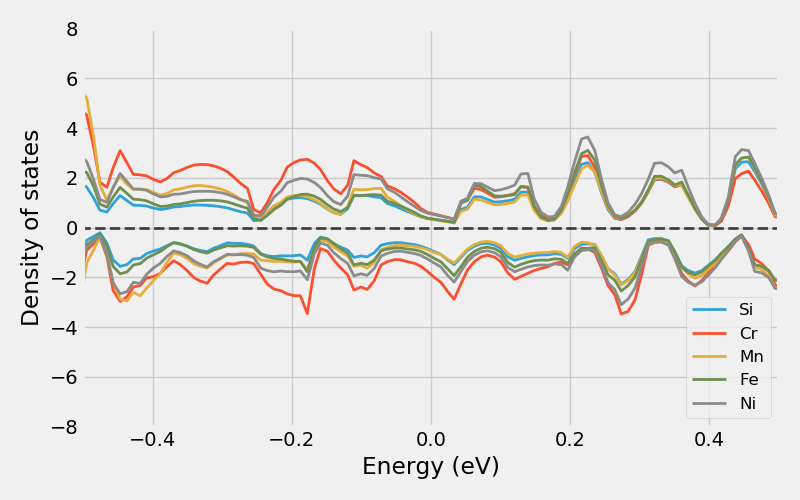
\includegraphics[width=.6\textwidth]{results/fesi2/permutations/ni7_PDOS.png}
	\caption{Projected density of states [states/eV] of \ch{Cr3Fe3Mn3Ni7Si32} around $E_F$}
\end{figure}

An important factor of these results is that because each composition alters simultaneous elements, interpreting and relating the results to a particular alteration is challenging. For example, is the result of the \ch{Cr5Fe3Mn5Ni3Si32} permutation a consequence of less Fe or increments to both Cr and Mn? Furthermore, is the large band gap in spin up of \ch{Cr3Fe3Mn7Ni3Si32} a product of increasing manganese or reducing the other elements? From the comparatively large gaps in spin up of \ch{Cr3Fe3Mn7Ni3Si32} and \ch{Cr3Fe5Mn5Ni3Si32} and the more present Cr states in spin up in the Cr rich permutations we here conclude that the band gap is related to lessening of chromium, more so than other effects. However we see from both \ch{Cr5Fe5Mn4Ni3Si32} and \ch{Cr3Fe3Mn3Ni7Si32} (figure 8.2) in addition to the manganese rich composition that Mn plays a vital role on the band gap of these structures. It's clear that the \ch{Cr3Fe5Mn5Ni3Si32} alloy manages to strike a balance between 3d elements that results in a specific interplay and correspondingly very promising properties. It could have been instructive to look at for example the pair distribution functions and compare to the equimolar system, but from the factors discussed in section 7.2.4, we leave this to future work. 

As stated previously, we have relied on the PBE GGA functional to determine the band gap, from its reliability and favorable computation cost. Nevertheless, we have conducted calculations with SCAN and HSE06 on some of the more promising structures. For instance, in SQS D of the \ch{Cr3Fe5Mn5Ni3Si32} alloy, we get lower values in both spin up and down with SCAN, specifically $E_\text{G, SCAN} ^\text{up}= 0.21$ eV and $E_\text{G, SCAN} ^\text{dw} = 0.08$ eV. On the other hand, we experience also in this case better cohesion between PBE and HSE06, with $E_\text{G, HSE06} ^\text{up} = 0.53$ eV and $E_\text{G, HSE06} ^\text{dw} = 0$ eV. In SQS B of the \ch{Cr3Fe3Mn7Ni3Si32} alloy, we found PBE band gaps equal to $E_\text{G, PBE} ^\text{up} = 0.47$ eV and $E_\text{G, PBE} ^\text{dw} = 0$ eV. Contrary, SCAN yields a small band gap in spin down of about 0.002 eV, and a 0 gap in spin up. Similarly, the HSE06 band gap of this structure is $E_\text{G, HSE06} ^\text{up} = 0.08$ eV and $E_\text{G, HSE06} ^\text{dw} = 0.11$ eV. Moreover, the HSE06 band gap of this structure is a defect band gap, thus we can get $E_\text{G, HSE06} ^\text{up, eigen}(0.01) = 0.18$ eV and $E_\text{G, HSE06} ^\text{dw, eigen}(0.01) = 0.16$ eV. 

\newpage
\section{High entropy silicides with cobalt/titanium}

The compositions in this section are deliberate combinations, intended to both investigate the role of individual elements in the \ch{(CrFeMnNi)Si2} system, and broaden our search of potential high-entropy silicides based on $\beta$-\ch{FeSi2}. In these alloys we replace Cr, Mn or Ni, with Co or Ti. Note that the alloys contain a total of 48 atoms as before, with equimolar distribution of 3d elements. In similar fashion to the preceding section, we begin by presenting in table 8.3, the mean and standard deviation of the total energy and magnetic moment of 5 distinct SQSs of each alloy

\begin{table}[H]
\centering
\begin{tabular}{@{}cccccc@{}}
\toprule
Composition           & \multicolumn{2}{c}{\begin{tabular}[c]{@{}c@{}}Toten \\ (eV)\end{tabular}} & \multicolumn{2}{c}{\begin{tabular}[c]{@{}c@{}}Mag\\ ($\mu_B$)\end{tabular}} & \begin{tabular}[c]{@{}c@{}}$E_{FPA}$\\ (eV)\end{tabular} \\ \midrule
                      & mean                                 & std                                & mean                                 & std                                  & mean                                                      \\ \midrule
\ch{(CrFeCoNi)Si2} & - 6.466                             & 0.006                             & 0.008                               & 0.016                               & -0.308                                                 \\
\ch{(CoFeMnNi)Si2} & - 6.473                             & 0.005                             & 0.000                               & 0.000                               & -0.355                                                 \\
\ch{(CrFeTiNi)Si2} & - 6.422                             & 0.009                             & 0.031                               & 0.029                               & -0.209                                                  \\
\ch{(CrFeMnTi)Si2} & -6.699                              & 0.007                             & 0.114                               & 0.064                               & -0.199                                                  \\
\ch{(CrFeMnCo)Si2} & -6.769                              & 0.003                             & 0.133                               & 0.033                               & -0.323                                                  \\ \bottomrule
\end{tabular}
\caption{Total energy, magnetic moment and formation energy of various compositions of the \ch{(CrFeMnNi)Si2} alloy, where Cr, Mn, or Ni is replaced by Co/Ti.}
\end{table}

In terms of the formation energy, we observe that cobalt evidently yield the most stable alloys, with \ch{(CoFeMnNi)Si2} at the top and and \ch{(CrFeCoNi)Si2} at the bottom. On the other side, both \ch{(CrFeTiNi)Si2} and \ch{(CrFeMnTi)Si2} where we introduce titanium in place of manganese and nickel respectively, results in the overall least stable compositions. A precise physical interpretation of the stability between compositions is challenging from the shallow analysis in this project, but we note that the two most stable alloys consists of the most chemically similar elements, with respect to properties such as electronegativity and atomic size. Accordingly, the least stable alloys are comprised of the most chemically dissimilar elements. This is in good agreement with the discussion in section 2.2, regarding phase formation of high-entropy alloys. Additionally, in the compositions discussed in the previous section, we observed that the most stable composition was \ch{Cr3Fe5Mn5Ni3Si32}, where the Cr proportion was reduced. In conjunction with the results of the titanium alloys above, we may suspect that smaller elements are ill-suited in these alloys based on \ch{FeSi2}.   

In line with the other compositions studied in this project, the magnetization is clearly related to chromium and manganese also in this case. This is seen by the overall lowest magnetic moments in the two compositions without these elements, and reversely the highest magnetic moments is found for compositions with both Cr and Mn. Comparing the magnetic moment of \ch{(CrFeCoNi)Si2} and \ch{(CoFeMnNi)Si2} it seems in our study that chromium is most responsible for the magnetic moment in these alloys. Furthermore we find that substituting Ni with both Ti and Co yields more magnetic compounds. As we have discussed previously, the uniqueness of each SQS makes it difficult to draw conclusion on the various properties. In table 8.4 below we list the magnetic moment of the utmost stable SQS in each alloy. Contrary to the mean value we find that \ch{(CrFeCoNi)Si2} similar to \ch{(CoFeMnNi)Si2} is nonmagnetic, moreover \ch{(CrFeMnTi)Si2} is less magnetic relative to both \ch{(CrFeMnCo)Si2} and \ch{(CrFeMnNi)Si2}. 

\begin{table}[H]
\centering
\begin{tabular}{@{}lc@{}}
\toprule
\multicolumn{1}{c}{Composition} & \begin{tabular}[c]{@{}c@{}}Magnetic moment\\ ($\mu_B$)\end{tabular} \\ \midrule
\ch{(CrFeCoNi)Si2}           & 0                                                                   \\
\ch{(CoFeMnNi)Si2}           & 0                                                                   \\
\ch{(CrFeTiNi)Si2}           & 0.065                                                              \\
\ch{(CrFeMnTi)Si2}           & 0.079                                                              \\
\ch{(CrFeMnCo)Si2}           & 0.167                                                              \\ \bottomrule
\end{tabular}
\caption{Magnetic moment of the most stable SQS of different Co/Ti alloys based on the \ch{(CrFeMnNi)Si2} alloy.}
\end{table}

\begin{table}[H]
\centering
\begin{tabular}{@{}ccccc@{}}
\toprule
\multicolumn{1}{l}{Composition}                   & $occ$                     & \begin{tabular}[c]{@{}c@{}}$E_\text{G} ^\text{up, eigen}$\\ (eV)\end{tabular} & \begin{tabular}[c]{@{}c@{}}$E_\text{G} ^\text{dw, eigen}$\\ (eV)\end{tabular} & \begin{tabular}[c]{@{}c@{}}$E_\text{G} ^\text{tot, eigen}$\\ (eV)\end{tabular} \\ \midrule
\multicolumn{1}{c|}{\multirow{3}{*}{\ch{(CrFeCoNi)Si2}}}                  & \multicolumn{1}{c|}{0.5}  & 0                                                                             & 0                                                                             & 0                                                                              \\
\multicolumn{1}{c|}{}                             & \multicolumn{1}{c|}{0.1}  & 0.001                                                                       & 0.040                                                                        & 0.001                                                                        \\
\multicolumn{1}{c|}{}                             & \multicolumn{1}{c|}{0.01} & 0.063                                                                         & 0.063                                                                         & 0.063                                                                          \\ \midrule
\multicolumn{1}{c|}{\multirow{3}{*}{\ch{(CrFeTiNi)Si2}}} & \multicolumn{1}{c|}{0.5}  & 0.007                                                                        & 0                                                                             & 0                                                                              \\
\multicolumn{1}{c|}{}                             & \multicolumn{1}{c|}{0.1}  & 0.061                                                                         & 0.009                                                                        & 0.009                                                                         \\
\multicolumn{1}{c|}{}                             & \multicolumn{1}{c|}{0.01} & 0.061                                                                         & 0.037                                                                         & 0.037                                                                          \\ \midrule
\multicolumn{1}{c|}{\multirow{3}{*}{\ch{(CoFeMnNi)Si2}}} & \multicolumn{1}{c|}{0.5}  & 0                                                                             & 0                                                                             & 0                                                                              \\
\multicolumn{1}{c|}{}                             & \multicolumn{1}{c|}{0.1}  & 0.004                                                                        & 0.004                                                                        & 0.004                                                                         \\
\multicolumn{1}{c|}{}                             & \multicolumn{1}{c|}{0.01} & 0.027                                                                        & 0.027                                                                        & 0.027                                                                         \\ \midrule
\multicolumn{1}{c|}{\multirow{3}{*}{\ch{(CrFeMnTi)Si2}}} & \multicolumn{1}{c|}{0.5}  & 0                                                                             & 0                                                                             & 0                                                                              \\
\multicolumn{1}{c|}{}                             & \multicolumn{1}{c|}{0.1}  & 0.021                                                                         & 0.001                                                                       & 0                                                                              \\
\multicolumn{1}{c|}{}                             & \multicolumn{1}{c|}{0.01} & 0.030                                                                          & 0.030                                                                          & 0.022                                                                          \\ \midrule
\multicolumn{1}{c|}{\multirow{3}{*}{\ch{(CrFeMnCo)Si2}}} & \multicolumn{1}{c|}{0.5}  & 0.461                                                                         & 0                                                                             & 0                                                                              \\
\multicolumn{1}{c|}{}                             & \multicolumn{1}{c|}{0.1}  & 0.607                                                                         & 0.022                                                                        & 0.022                                                                         \\
\multicolumn{1}{c|}{}                             & \multicolumn{1}{c|}{0.01}                      & 0.607                                                                         & 0.025                                                                        & 0.025                                                                         \\ \bottomrule
\end{tabular}
\caption{The band gap in spin up/down and total of the most stable SQS of high-entropy silicides with cobalt/titanium. Calculated from eigenvalues with different occupancy cutoff $occ$. }
\end{table}

Thus, based on the utmost stable configurations we can state that replacing either Cr or Mn (with Co), removes the magnetic moment of the alloy. Furthermore we find that the magnetic moment is reduced when Ni is substituted with Ti, and increased by Co. However, while substituting manganese with Co yields a nonmagnetic alloy, Ti for Mn only slightly reduces the magnetic moment. 

In regards to the band gap, we discover that the majority of alloys are metals. In table 8.5, we list the band gap of the most stable SQS of each composition, where the band gap is determined from the eigenvalues at different occupancy cutoff $occ$ values, to underline the effect of defect states on the band gaps. By increasing the criteria, in other words only consider states with occupancy above a certain threshold, the band gap materializes with $occ = 0.1$ and converges to around $0.02 - 0.06$ eV depending on composition at $occ = 0.01$.
 
Aside from a very narrow spin up band gap in the \ch{(CrFeTiNi)Si2} alloy, we only report a sizable band gap of these alloys in the \ch{CrFeMnCoSi2} composition of around 0.5 eV in spin up. In figure 8.3 we plot the projected density of states of this structure. As was generally the case for the Cr:Fe:Mn:Ni:Si alloys, this structure displays a dominant number of manganese states in spin down at energies just above $E_F$, and a large number of Cr states right below $E_F$ in spin up. Analog to the most stable supercell of the \ch{Cr5Fe5Mn3Ni3Si32} alloy discussed in section 8.1, the presence of defect states in the spin up band gap of \ch{CrFeMnCoSi2}, results in small finite DOS at the Fermi energy, and the band gap calculated from the eigenvalues is shifted above $E_F$, resembling that of a doped material.  
  
\begin{figure}[H]
\centering
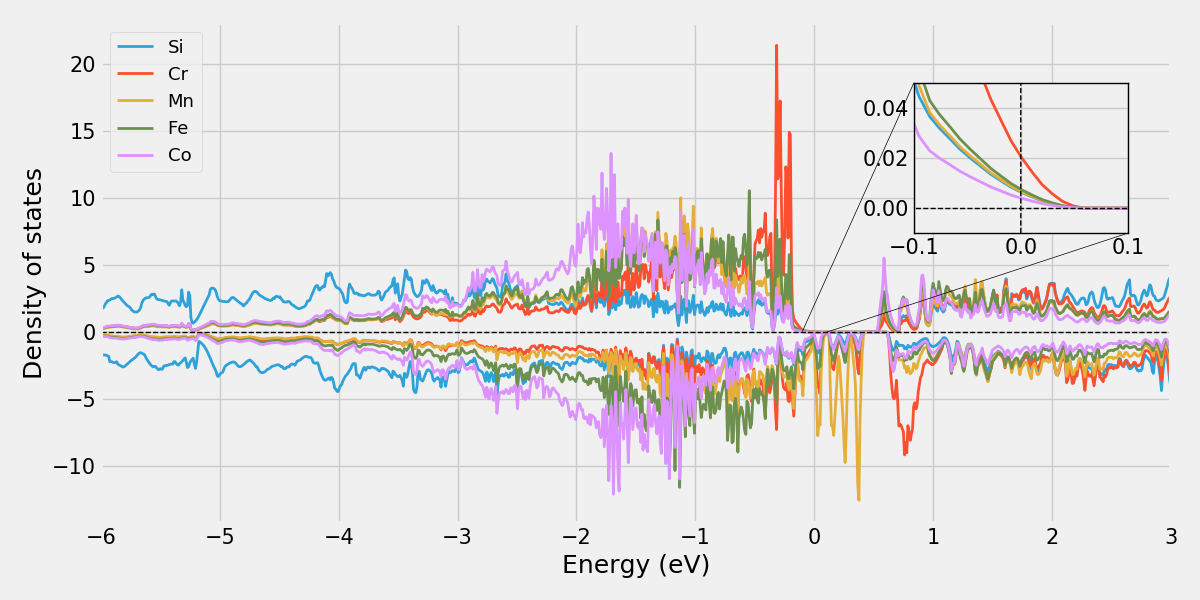
\includegraphics[width=\textwidth]{results/fesi2/composistions/crfemnco_PDOS.png}
\caption{Projected density of states [states/eV] of \ch{(CrFeMnCo)Si2}.}
\end{figure}

The PDOSs of the other four alloys is displayed in figure 8.4. In agreement with the values listed in table 8.5, we observe from the PDOS that these are metallic compounds with finite DOS at $E_F$ in both spins. 
 
\begin{figure}[H]
\begin{subfigure}{.5\textwidth}
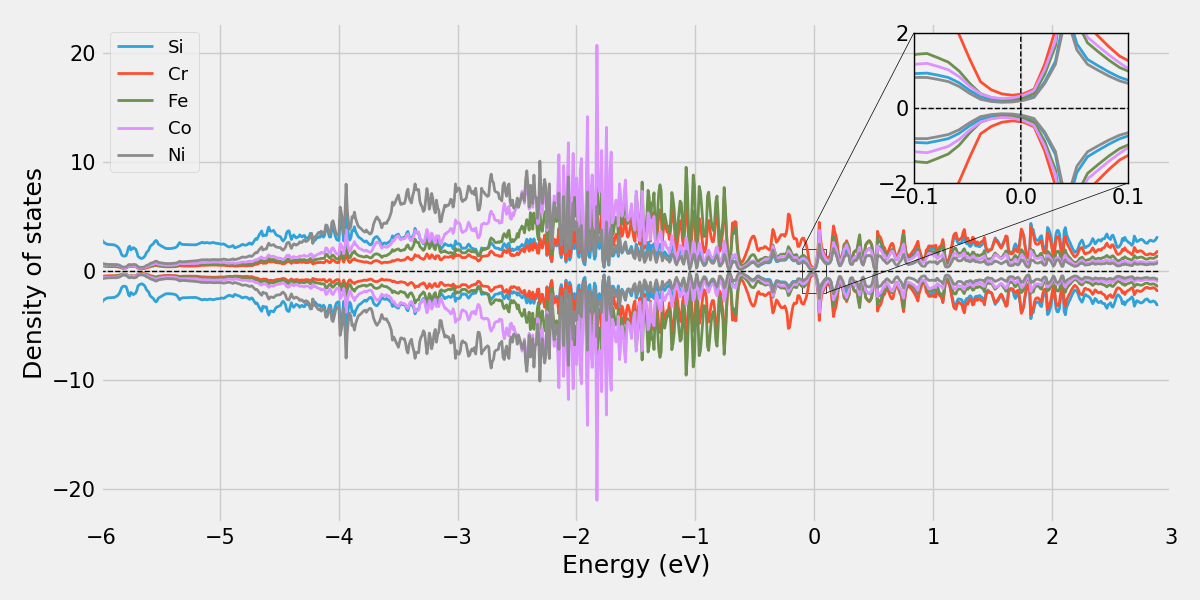
\includegraphics[width=\textwidth]{results/fesi2/crfeconi_PDOS.png}
\caption{\ch{Cr4Fe4Co4Ni4Si32}}
\end{subfigure}
\begin{subfigure}{.5\textwidth}
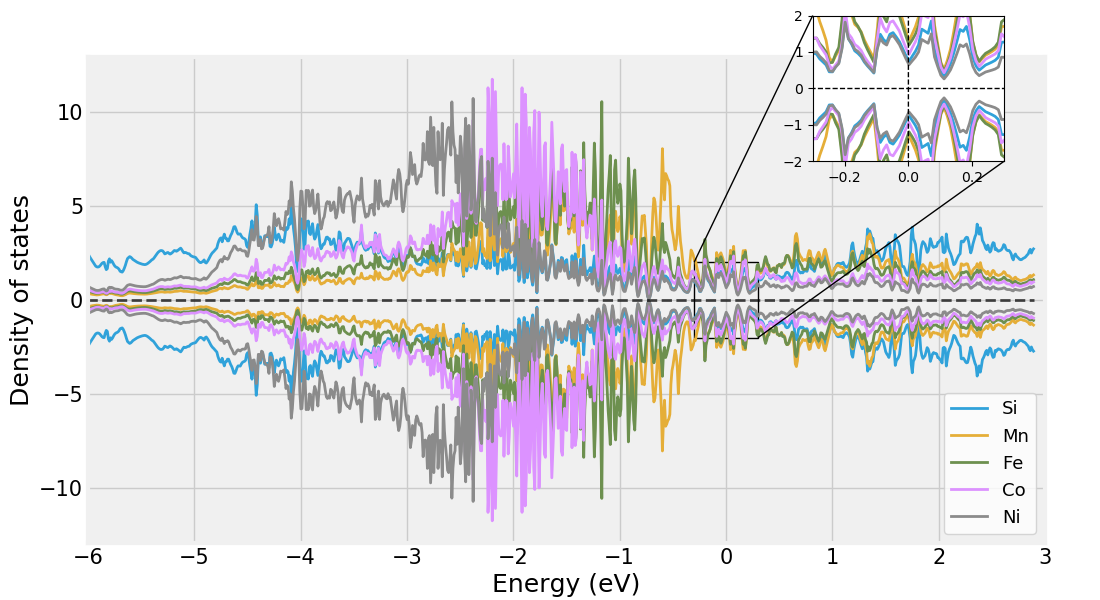
\includegraphics[width=\textwidth]{results/fesi2/cofemnni_PDOS.png}
\caption{\ch{Co4Fe4Mn4Ni4Si32}}
\end{subfigure}
\begin{subfigure}{.5\textwidth}
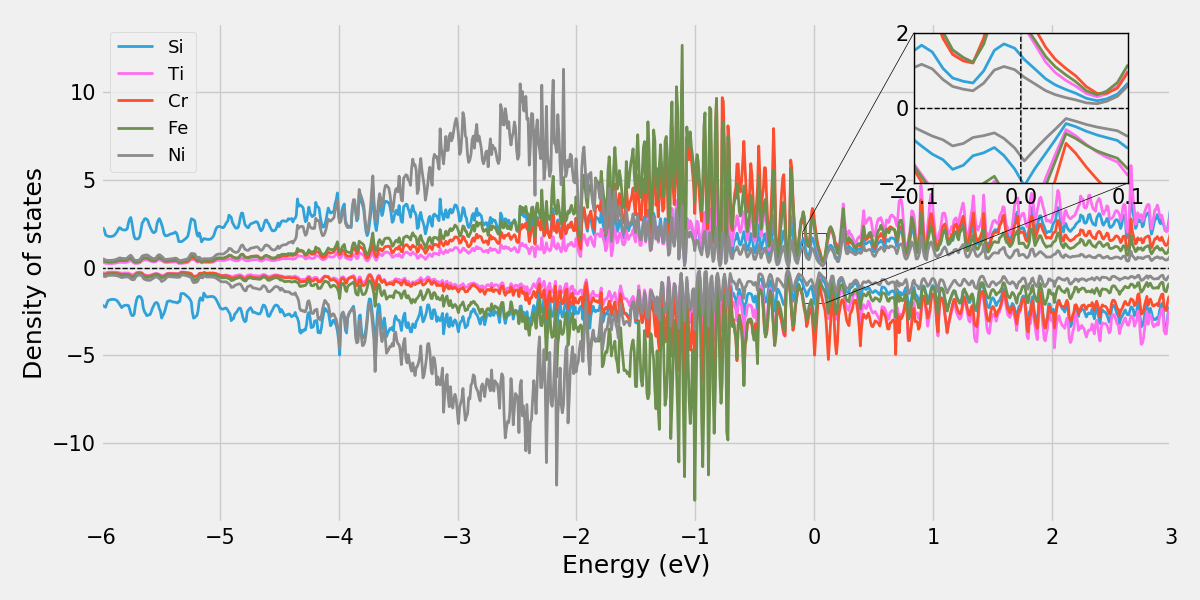
\includegraphics[width=\textwidth]{results/fesi2/crfetini_PDOS.png}
\caption{\ch{Cr4Fe4Ti4Ni4Si32}}
\end{subfigure}
\begin{subfigure}{.5\textwidth}
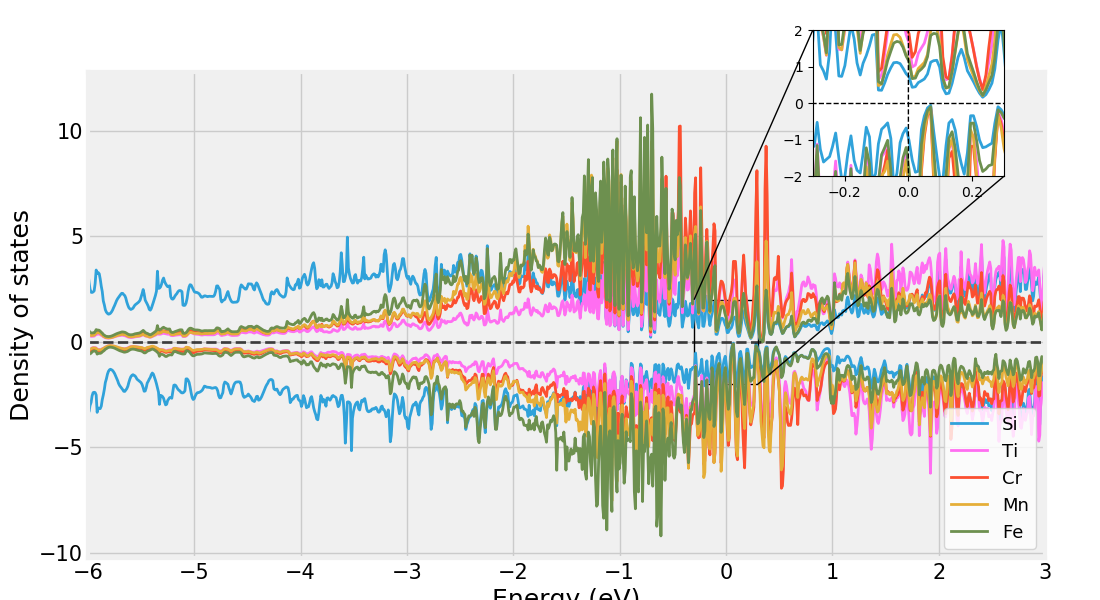
\includegraphics[width=\textwidth]{results/fesi2/crfemnti_PDOS.png}
\caption{\ch{Cr4Fe4Mn4Ti4Si32}}
\end{subfigure}
\caption{Projected density of states [states/eV] of Co/Ti alloys based on the \ch{(CrFeMnNi)Si2} alloy.}
\end{figure}

Above we have evaluated the band gap of the different alloys based on the most stable configuration. Considering all five configurations, we find that the band gap is more or less consistent between supercells of \ch{(CrFeCoNi)Si2},  \ch{(CrFeMnTiSi2)}, \ch{(CrFeTiNi)Si2} and \ch{(CrFeMnCo)Si2}. Contrary, in the \ch{CoFeMnNiSi2} alloy we find very narrow total band gaps in two lesser stable configurations (SQS A and E) of 0.03 eV and 0.006 eV respectively. The density of states of these structures are displayed in figure 8.5.

\begin{figure}[H]
\begin{subfigure}{.5\textwidth}
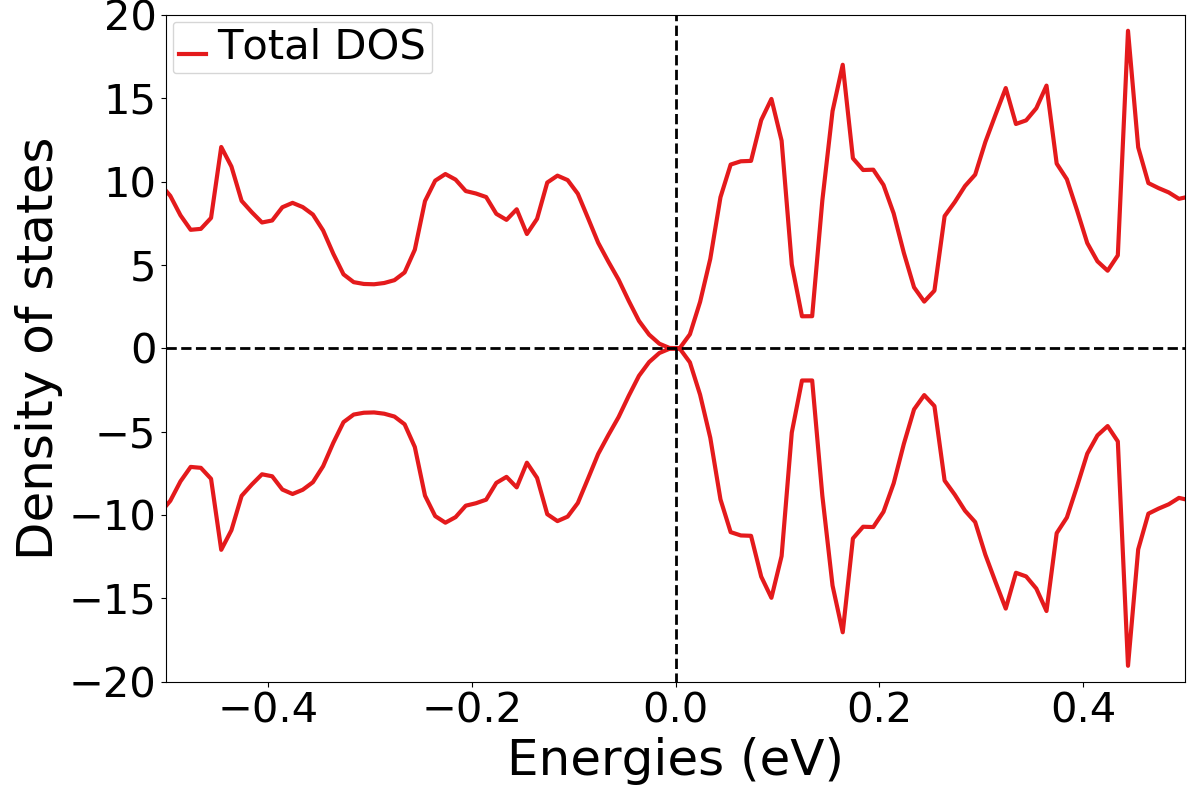
\includegraphics[width=\textwidth]{results/fesi2/composistions/cofemnni_E_DOS.png}
\caption{SQS A}
\end{subfigure}
\begin{subfigure}{.5\textwidth}
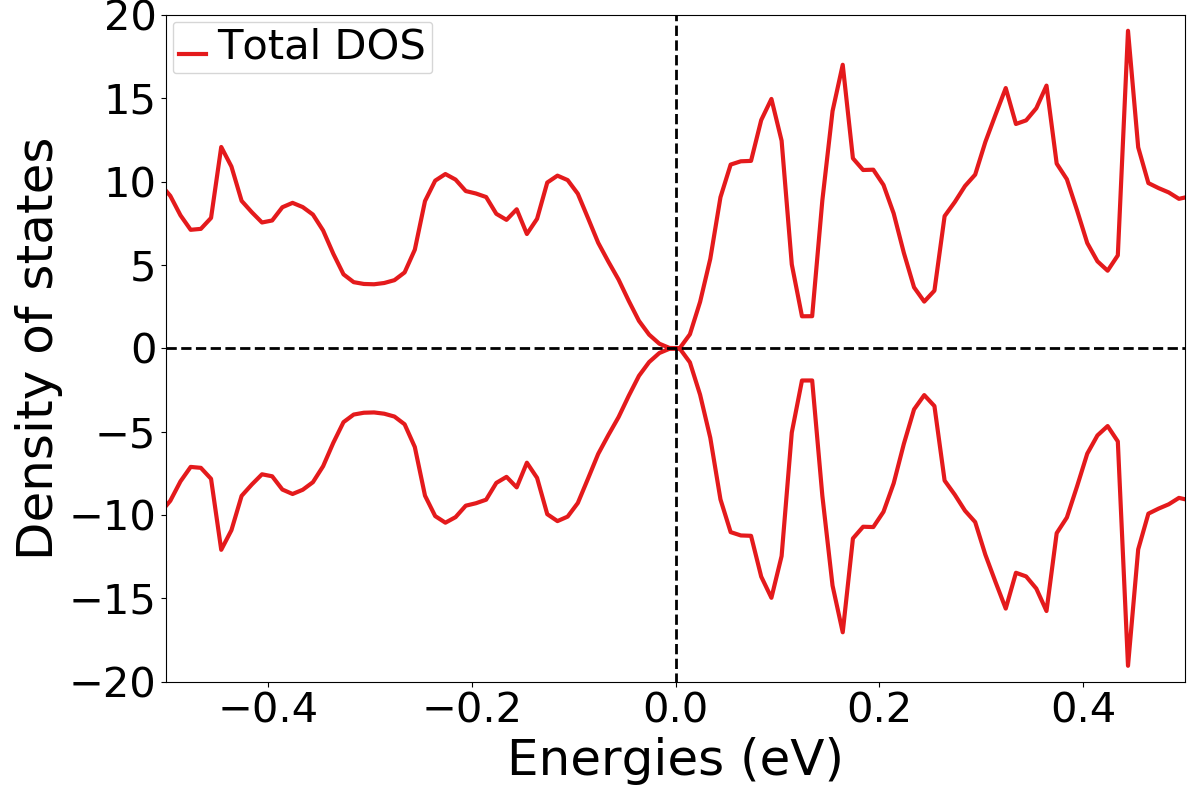
\includegraphics[width=\textwidth]{results/fesi2/composistions/cofemnni_E_DOS.png}
\caption{SQS E}
\end{subfigure}
\caption{Density of states [states/eV] of SQS A and E of \ch{(CoFeMnNi)Si2}.}
\end{figure} 

\newpage
\section{Negative systems}

In the above sections we have observed that aside from the \ch{(CrFeMnNi)Si2} alloy, we have limited success in locating semiconducting alloys when moving away from the Cr:Fe:Mn:Ni:Si system. In addition to the alloys disused above, we have carried out similar simulations on other alloys not included in this report. In most of these alloys we experienced limited or no success with respect to the band gap. All five SQSs of a \ch{(ScVMnZn)Si2} alloy based on \ch{FeSi2} turned out metallic. In \ch{(VMnFeCu)Si2}, we found one supercell with a defect band gap of 0.007 eV. Furthermore, we tested various four-element compositions such as \ch{Cr6Co6Ni4Si32}, \ch{Cr6Fe6Co4Si32}, \ch{Cr6Fe6Ni4Si32} and \ch{Fe6Co6Ni4Si32}. Out of these four compositions and corresponding 20 total SQSs, noteworthy we find a defect band gap of 0.15 eV in the spin up direction in one supercell of \ch{Cr6Fe6Co4Si32}, and a spin up band gap of 0.27 eV in \ch{Cr6Fe6Ni4Si32}. In the latter, we observed smaller single spin band gaps in additional configurations as well. The other two compositions were metallic across all tested supercells.    

Moreover, we attempted to replicate the Cr:Fe:Mn:Ni:Si system based on other silicides, such as hexagonal \ch{CrSi2}, trigonal \ch{Fe2Si}, and tetragonal and orthorombic \ch{Mn4Si7}. Unfortunately, these systems were generally much more difficult to simulate, and of the ones we managed showed very minimal indications of a band gap, compared to the \ch{FeSi2} based alloys. 
